% ==============================================================================================
\chapter{Moving load on an elastic halfspace} \label{ch:moving_load_halfspace}
% ==============================================================================================

% ----------------------------------------------------------------------------------------------
\section{Introduction}
% ----------------------------------------------------------------------------------------------
This benchmark compares the STEM numerical solution against the analytical solution,
for a moving load travelling on an elastic halfspace.

The analytical solution is presented in~\cite{Liao_Teng_Yeh_2005}.
The analytical solution provides closed-form expressions for the vertical displacement below the surface of the
halfspace, enabling a direct time-history comparison against the numerical model.

% ----------------------------------------------------------------------------------------------
\section{Model Description}
% ----------------------------------------------------------------------------------------------

% ..............................................................................................
\subsection{Geometry, mesh and loading}
% ..............................................................................................
The soil domain is modelled as a three-dimensional block representing the halfspace, with the following dimensions:
height \qty{10}{\meter}, width \qty{10}{\meter} and length \qty{20}{\meter}.
The soil is discretised with second-order tetrahedral elements, using an average element size of \qty{0.50}{\meter}.
An overview of the geometry and mesh adopted for the analysis is shown in
Figure~\ref{fig:moving_load_halfspace_mesh}.

The moving load is modelled as a vertical point load travelling along the z-direction at a constant speed of
\qty{10}{\meter\per\second}.
The load has a magnitude of \qty{1000}{\kilo\newton}.

The nodes at the sides of the soil have absorbing boundaries at the free ends, and with fixed boundary conditions
on the perpendicular plane along the axis of symmetry.
At the bottom the soil is assumed to be fixed.


\begin{figure}
	\centering
	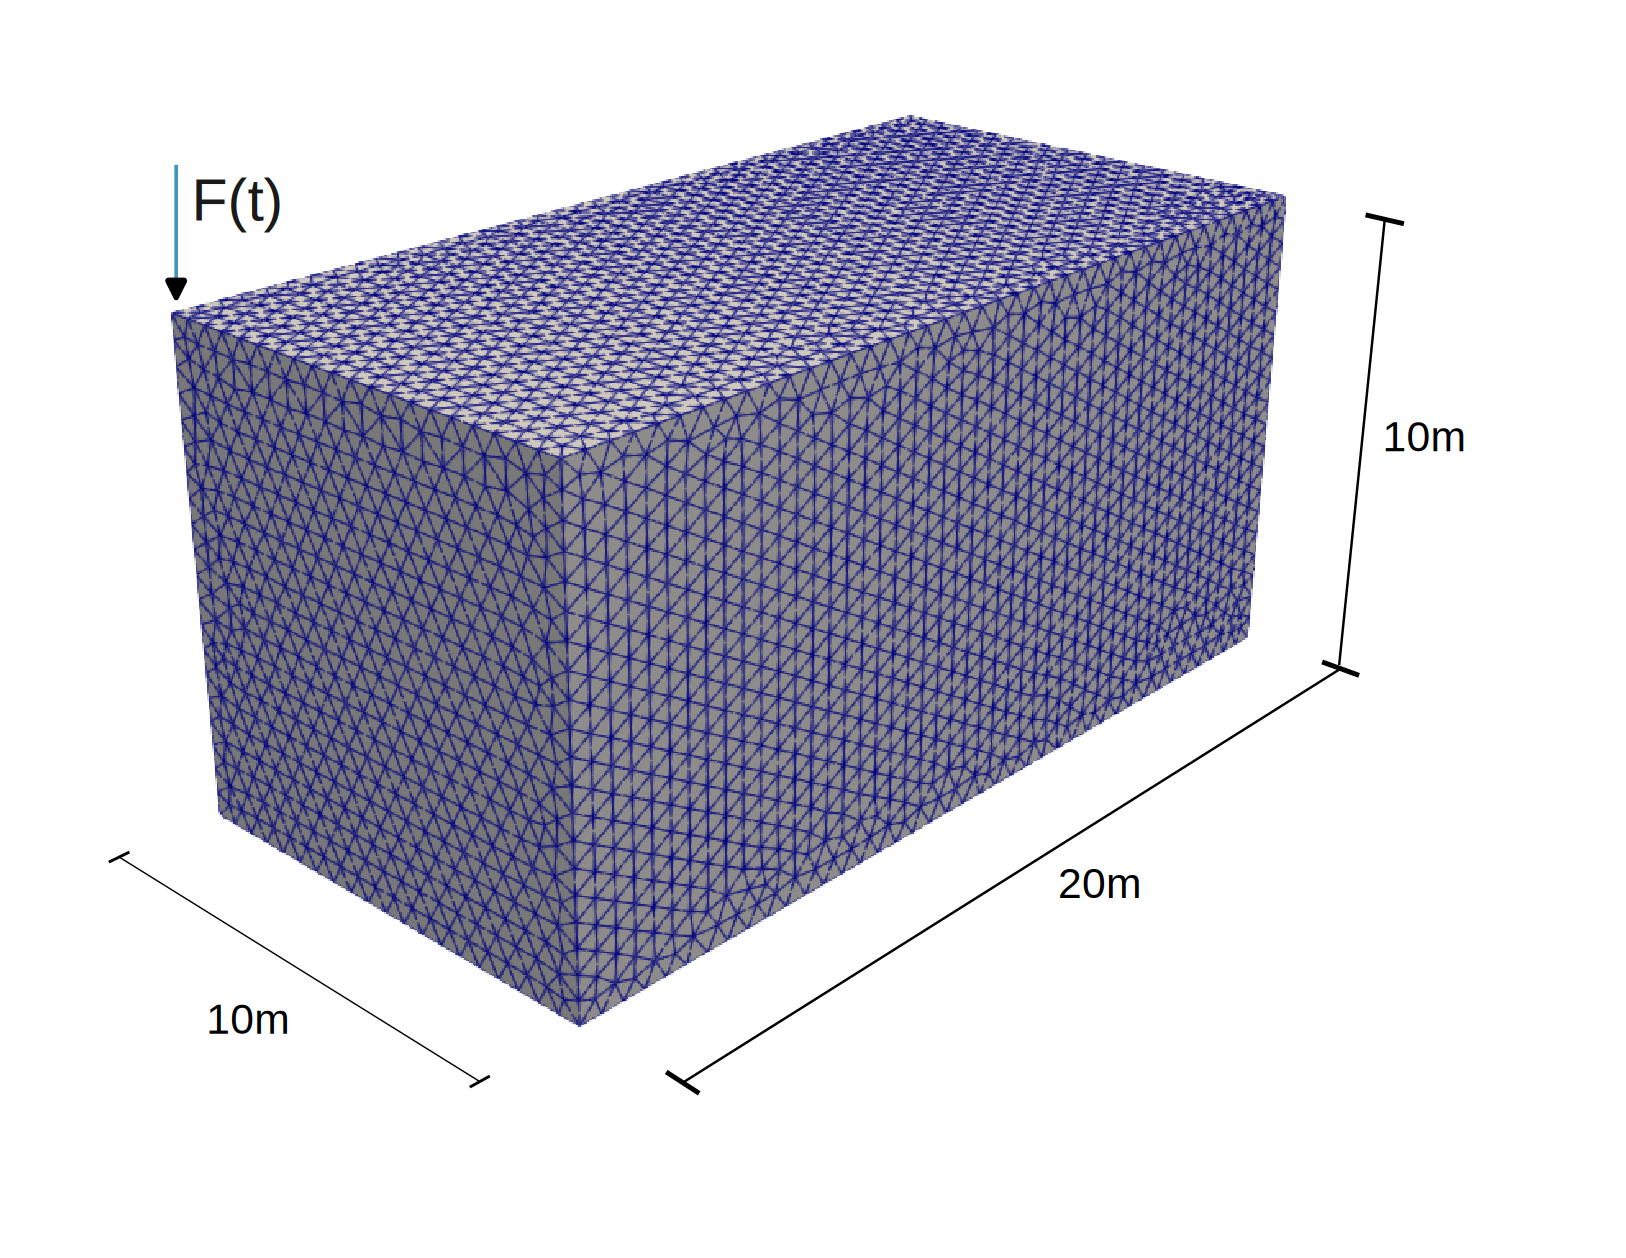
\includegraphics[width=0.75\textwidth]{moving_load_halfspace/mesh.pdf}
	\caption{Geometry and mesh adopted for the moving load on an elastic halfspace benchmark.}
	\label{fig:moving_load_halfspace_mesh}
\end{figure}

% ..............................................................................................
\subsection{Materials and numerical parameters}
% ..............................................................................................
The soil is modelled as a one-phase continuum with a linear elastic constitutive law, with the
following parameters:

\begin{itemize}[noitemsep,topsep=0pt,parsep=0pt,partopsep=0pt]
	\item Young's modulus: \qty{30}{\mega\pascal},
	\item Poisson ratio: \qty{0.2}{},
	\item Solid density: \qty{2000}{\kilogram\per\meter\cubed},
\end{itemize}

% The material damping is set to zero, in order to allow a direct comparison against the analytical solution.
Material damping is included via Rayleigh damping, with parameters that provide a damping ratio of
\qty{1}{\percent} at \qty{1}{\hertz} and \qty{80}{\hertz}.

The dynamic analysis is performed over a \qty{1.5}{\second} time window, with a time step of \qty{0.01}{\second}.
The system of equations is solved using the Newmark time integration~\cite{Newmark_1959} scheme with
parameters $\beta = 0.25$ and $\gamma = 0.5$.


% ----------------------------------------------------------------------------------------------
\section{Results}
% ----------------------------------------------------------------------------------------------
Figure~\ref{fig:moving_load_halfspace_results} presents the time history of the
vertical displacement for a point located in the middle of the model at a depth of \qty{1}{\meter}
(coordinates (5, 5, -1)).
The figure compares the numerical STEM results against the analytical solution.
If follows that there is an agreement between both solutions, demonstrating the accuracy of the STEM
for this type of dynamic loading condition. The STEM solution exhibits some high frequency content,
which is not present in the analytical solution, and which are related to the domain truncation, and boundary conditions
adopted in the numerical model (the analytical solution assumes an infinite halfspace).

\begin{figure}[h]
	\centering
	\includegraphics[width=0.8\textwidth]{moving_load_halfspace/time_history.pdf}
	\caption{Comparison of the vertical displacement time history at a point located in the middle of the model at
	 a depth of \qty{1}{\meter} (coordinates (5, 5, -1)).}
	\label{fig:moving_load_halfspace_results}
\end{figure}

